\documentclass[a4paper,12pt]{article}
\usepackage[utf8]{inputenc}
\usepackage[italian]{babel}
\usepackage{amsmath, amssymb}
\usepackage{graphicx}
\usepackage{geometry}
\usepackage{fancyhdr}
\usepackage{physics}
\usepackage{siunitx}
\usepackage{titlesec}
\usepackage{xcolor}
\usepackage{float}
\usepackage{setspace}
\geometry{margin=2.5cm}
\setlength{\parindent}{0pt}
\begin{document}

\begin{center}
    \Large\textbf{Il pendolo conico}\\[4pt]
    \normalsize Fisica: principi della dinamica - moto circolare uniforme
\end{center}

\vspace{0.5cm}

\begin{figure}[H]
    \centering
    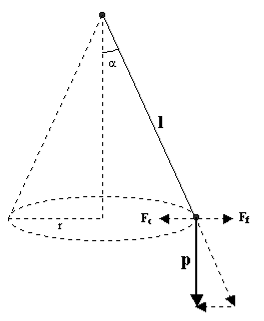
\includegraphics[width=0.35\textwidth]{../../immagini/pendconico.png}
 
\end{figure}

\section*{Analisi delle forze}

\subsection*{Scomposizione della tensione}

La tensione \(T\) viene scomposta in due componenti:

\begin{itemize}
    \item \textbf{Componente verticale} \(\,T\cos\theta\): bilancia la forza peso \(mg\), mantenendo la massa in equilibrio verticale.
    \item \textbf{Componente orizzontale} \(\,T\sin\theta\): questa è la forza centripeta che causa il moto circolare, diretta verso il centro del cerchio di rotazione.
\end{itemize}

\subsection*{Equilibrio delle forze}

\textbf{Verticale:}
\[
T\cos\theta = mg.
\]

\textbf{Orizzontale:}
\[
T\sin\theta = F_{c},
\]
dove \(F_{c}\) è la forza centripeta. Poiché
\[
F_{c} = m\omega^{2} r,
\]
(con \(r\) raggio del cerchio di rotazione) si ottiene:
\[
T\sin\theta = m\omega^{2} r.
\]

\section*{Forze centripeta e centrifuga}

\textbf{Forza centripeta:} è una forza reale, risultante delle forze applicate (in questo caso, la componente orizzontale della tensione). La sua funzione è quella di attrarre la massa verso il centro del moto circolare, ed è necessaria per mantenere la traiettoria circolare.

\medskip

\textbf{Forza centrifuga:} è una forza apparente o fittizia che compare in un sistema di riferimento non inerziale (un sistema in rotazione). Per un osservatore solidale con la massa del pendolo, questa forza percepita è diretta verso l’esterno, bilanciando la tensione e mantenendo costante l’inclinazione del pendolo \(\theta\). In un sistema di riferimento inerziale, la forza centrifuga non esiste.

\end{document}
